\documentclass[border=2mm]{standalone}
\usepackage{tikz}

\begin{document}

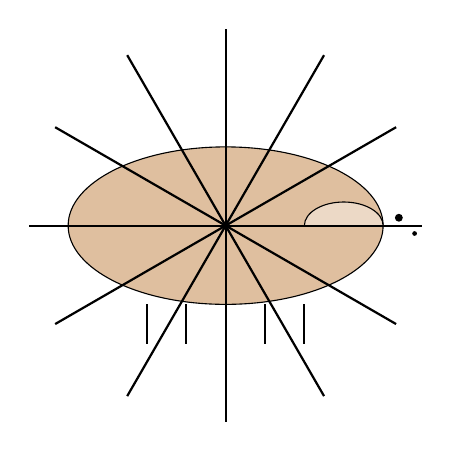
\begin{tikzpicture}
    % Ciało jeża
    \draw[fill=brown!50] (0,0) ellipse (2 and 1);

    % Głowa jeża
    \draw[fill=brown!30] (2,0) arc (0:180:0.5 and 0.3);

    % Oko
    \fill[black] (2.2,0.1) circle (0.05);

    % Nos
    \fill[black] (2.4,-0.1) circle (0.03);

    % Kolce
    \foreach \i in {0,30,60,...,360} {
        \draw[thick] (0,0) -- (\i:2.5);
    }

    % Nogi
    \draw[thick] (-1,-1) -- (-1,-1.5);
    \draw[thick] (-0.5,-1) -- (-0.5,-1.5);
    \draw[thick] (0.5,-1) -- (0.5,-1.5);
    \draw[thick] (1,-1) -- (1,-1.5);
\end{tikzpicture}

\end{document}